\section{Conceptual Attention}
\label{sec:main-ca}

Motivated by the preceding refine-or-repair theory, we propose Conceptual Attention (CA) as a fixed-capacity attention replacement. The layer used in our main experiments allocates a bounded bank of concept identities, keeps all slots active, disables graph edges, and updates only a concept-value memory during the forward pass. A concept is an operational address for a prediction-relevant information cell, not necessarily a human-semantic category. The graph-growing and edge-gated CA variant in the appendix is the dynamic refinement implementation; the main MQAR and CoM experiments use the fixed-bank, edge-free path.

Operationally, CA is linear attention over a learned concept bank. Standard causal attention stores one key-value pair per prefix token. CA instead stores a fixed number $C$ of concept addresses and a recurrent value table over those addresses. For head $h$ and concept slot $j$, the layer has a unit address
\begin{align*}
a_{hj}\in\mathbb{R}^{d_a},\qquad \|a_{hj}\|_2=1 .
\end{align*}
In the code path used for CoM and MQAR, these addresses are trainable layer parameters initialized as random unit vectors. They are \emph{not} online sequence state: they are shared across examples and updated only by ordinary training. The online state for a sequence is the concept-value memory
\begin{align*}
M_t\in\mathbb{R}^{H\times C\times d_v^c}.
\end{align*}
Thus the persistent runtime state per layer is
\begin{align*}
S_{\rm CA}=C H d_v^c ,
\end{align*}
independent of prefix length. With delayed writes, the implementation also keeps a small key buffer of size $O(\delta H d_a)$; the language-model setting uses $\delta=0$.

\begin{figure}[t]
\centering
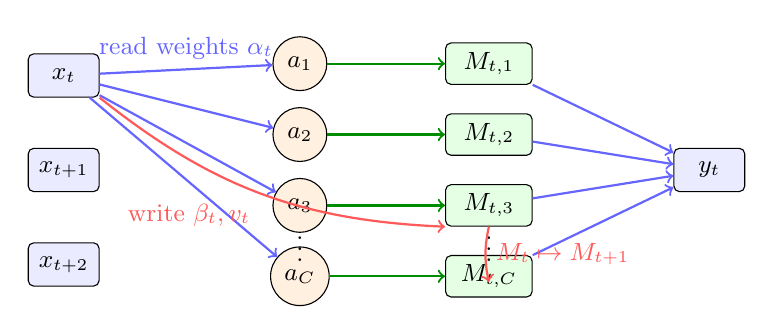
\begin{tikzpicture}[
  font=\small,
  token/.style={draw, rounded corners=2pt, minimum width=0.9cm, minimum height=0.55cm, fill=blue!8},
  concept/.style={draw, circle, minimum size=0.62cm, fill=orange!12},
  mem/.style={draw, rounded corners=2pt, minimum width=1.1cm, minimum height=0.48cm, fill=green!10},
  arrow/.style={->, thick}
]
\node[token] (x1) at (0,1.2) {$x_t$};
\node[token] (x2) at (0,0) {$x_{t+1}$};
\node[token] (x3) at (0,-1.2) {$x_{t+2}$};

\node[concept] (c1) at (3,1.35) {$a_1$};
\node[concept] (c2) at (3,0.45) {$a_2$};
\node[concept] (c3) at (3,-0.45) {$a_3$};
\node[concept] (c4) at (3,-1.35) {$a_C$};
\node at (3,-0.9) {$\vdots$};

\node[mem] (m1) at (5.4,1.35) {$M_{t,1}$};
\node[mem] (m2) at (5.4,0.45) {$M_{t,2}$};
\node[mem] (m3) at (5.4,-0.45) {$M_{t,3}$};
\node[mem] (m4) at (5.4,-1.35) {$M_{t,C}$};
\node at (5.4,-0.9) {$\vdots$};

\node[token] (y) at (8.2,0) {$y_t$};

\draw[arrow, blue!60] (x1) -- node[above] {read weights $\alpha_t$} (c1);
\draw[arrow, blue!60] (x1) -- (c2);
\draw[arrow, blue!60] (x1) -- (c3);
\draw[arrow, blue!60] (x1) -- (c4);
\draw[arrow, green!55!black] (c1) -- (m1);
\draw[arrow, green!55!black] (c2) -- (m2);
\draw[arrow, green!55!black] (c3) -- (m3);
\draw[arrow, green!55!black] (c4) -- (m4);
\draw[arrow, blue!60] (m1) -- (y);
\draw[arrow, blue!60] (m2) -- (y);
\draw[arrow, blue!60] (m3) -- (y);
\draw[arrow, blue!60] (m4) -- (y);

\draw[arrow, red!65, bend right=18] (x1.south east) to node[below left] {write $\beta_t,v_t$} (m3.south west);
\draw[arrow, red!65, bend right=12] (m3.south) to node[right] {$M_t\mapsto M_{t+1}$} ++(0,-0.7);
\end{tikzpicture}
\caption{Conceptual Attention replaces token-indexed KV memory with a fixed learned concept bank and a mutable concept-value table. Tokens attend to concept identities for reads, then update the concept values by a retained forward write.}
\label{fig:ca-concept-bank}
\end{figure}

\paragraph{Token recurrence.}
Given hidden states $x_t\in\mathbb{R}^{d_{\rm model}}$, CA forms normalized read queries and write keys, concept values, and retention rates:
\begin{align*}
q_{th}=\operatorname{normalize}(Q_hx_t),\qquad
k_{th}=\operatorname{normalize}(K_hx_t),
\end{align*}
\begin{align*}
v_{th}=V_hx_t,\qquad
\rho_{th}=\exp(-\lambda_{th})\in(0,1].
\end{align*}
Let $\gamma>0$ be the learned read/write scale. Token $t$ first reads the current concept memory:
\begin{align*}
\alpha_{thj}
=
\operatorname{softmax}_{j}(\gamma q_{th}^{\top}a_{hj}),
\qquad
z_{th}=\sum_{j=1}^{C}\alpha_{thj}M_{t,hj},
\qquad
y_t=O[z_{t1};\ldots;z_{tH}].
\end{align*}
Then it updates the memory. For a write delay $\delta\ge0$, define $\bar k_{th}=k_{t-\delta,h}$ and a valid-write mask $m_t=\mathbf{1}\{t\ge\delta\}$. The language-model experiments use $\delta=0$; MQAR can use $\delta=1$ to bind a value token to the preceding key token. The write distribution is
\begin{align*}
\beta_{thj}
=
\operatorname{softmax}_{j}(\gamma \bar k_{th}^{\top}a_{hj}),
\end{align*}
and the read-before-write recurrence is
\begin{align}
M_{t+1,hj}
=
\rho_{th}M_{t,hj}
+m_t\beta_{thj}v_{th}.
\label{eq:ca-token-recurrence}
\end{align}
This is the algorithm implemented by the streaming \texttt{step} API: each token consumes and returns a constant-size recurrent state, exactly as in linear attention or state-space decoding.

\begin{proposition}[Linear-time CA state]
\label{prop:main-ca-state}
Fix the learned CA parameters and concept addresses. For any prefix length $T$, all prefix dependence needed by future CA outputs is contained in $M_T$ and, when $\delta>0$, the delayed-key buffer. The per-layer online state is $C H d_v^c+O(\delta H d_a)$ and the autoregressive update cost is $O(HC(d_a+d_v^c))$ per token, independent of $T$.
\end{proposition}

\begin{proof}[Proof sketch]
Equation~\eqref{eq:ca-token-recurrence} is Markov in $(M_t,\bar k_t)$. The next output reads only $M_t$ and the current hidden state, and the next memory is a deterministic function of the same state and current projections. Induction over tokens gives the claim. The memory tensor has $H C d_v^c$ scalars and the delayed-write buffer stores only $\delta$ normalized keys.
\end{proof}

\paragraph{Parallel training by chunk scan.}
The token recurrence is sequential, but it has the same affine-scan structure used by linear recurrent attention. For token $t$ define the additive update
\begin{align*}
U_{t,hj}=m_t\beta_{thj}v_{th}.
\end{align*}
The transition $M\mapsto \rho_t M+U_t$ is an affine map. For a chunk $b=[s,e)$, the code computes the exact chunk summary
\begin{align*}
R_{b,h}=\prod_{t=s}^{e-1}\rho_{th},
\qquad
U_{b,hj}=\sum_{t=s}^{e-1}
\left(\prod_{u=t+1}^{e-1}\rho_{uh}\right)
m_t\beta_{thj}v_{th}.
\end{align*}
The summary maps the entering memory to the exiting memory:
\begin{align*}
M_{e,hj}=R_{b,h}M_{s,hj}+U_{b,hj}.
\end{align*}
Chunk summaries compose associatively:
\begin{align*}
(R_2,U_2)\odot(R_1,U_1)
=
(R_2R_1,\ U_2+R_2U_1),
\end{align*}
where $R$ broadcasts over concepts and values. Therefore all chunk-entry memories can be computed by an exclusive associative scan over $(R_b,U_b)$.

After the scan recovers the entering memory for each chunk, the chunk read kernel also includes all earlier writes inside the same chunk. For token $t\in[s,e)$,
\begin{align*}
M_{t,hj}
=
\left(\prod_{u=s}^{t-1}\rho_{uh}\right)M_{s,hj}
+
\sum_{r=s}^{t-1}
\left(\prod_{u=r+1}^{t-1}\rho_{uh}\right)
m_r\beta_{rhj}v_{rh}.
\end{align*}
The output read uses this $M_t$. Thus chunking changes the evaluation order and exposes parallel dense kernels, but it is mathematically equivalent to the token recurrence in Equation~\eqref{eq:ca-token-recurrence}. The block size is a tiling parameter, not a modeling approximation.

\begin{algorithm}[H]
\caption{\textsc{CAForward} as implemented}
\label{alg:ca-forward}
\begin{algorithmic}[1]
\State \textbf{Input:} hidden states $x_{1:L}$, learned concept identities $a_{1:C}$, initial memory $M_0=0$
\State project all $q_t,k_t,v_t,\rho_t$ and normalize $q_t,k_t,a_j$
\State form dense concept read weights $\alpha_t$ and write weights $\beta_t$
\State split the sequence into chunks of size $B$
\State build exact affine summaries $(R_b,U_b)$ for all chunks in parallel
\State compute chunk-entry memories by exclusive associative scan over $(R_b,U_b)$
\State for each chunk, compute exact read-before-write token outputs using its entry memory and within-chunk prior writes
\State \Return output projection of the multi-head concept reads
\end{algorithmic}
\end{algorithm}

\paragraph{Trainable retention.}
The factor $\rho_{th}$ controls how much old concept memory survives a token write. CA computes positive decay rates $\lambda_{th}$ from the hidden state. Our default parameterization uses a PoST-style ordered spectrum for base decay rates,
\begin{align*}
A_h=A_0+\sum_{i<h}\operatorname{softplus}(\Delta_i),
\end{align*}
combined with learned input-dependent step sizes and optional position-adaptive scaling. This gives CA a trainable forgetting spectrum, but the recurrence acts on concept-value memory rather than a token-indexed KV cache.

\paragraph{Training and inference.}
During training, slow parameters are optimized by ordinary backpropagation through the read weights $\alpha$, write weights $\beta$, values $v_t$, retention factors $\rho_t$, output projection, and the scan recurrence. During inference, model weights and concept identities are fixed. The only changing state is the forward-updated concept memory $M_t$ and the optional delayed-key buffer. This is the sense in which CA performs test-time learning: future predictions condition on a memory learned from the observed prefix, without running backpropagation at inference time.

This fixed-bank recurrence is the additive repair form used in the reported experiments. CoM replaces the unnormalized value write by closed-form sufficient-statistic updates in the same concept coordinates, such as responsibility-weighted counts, means, or recursive least-squares statistics. That extension preserves the same read/write concept interface while making the test-time update explicitly gradient-free and consequence-aligned.

\paragraph{Relation to ordinary attention.}
Standard causal attention computes
\begin{align*}
\operatorname{Attn}(X)_t
=
\sum_{s<t}\operatorname{softmax}_s(q_t^\top K_s)V_s,
\end{align*}
where the memory basis is the set of prefix token positions. CA computes
\begin{align*}
\operatorname{CA}(X)_t
=
\sum_{j=1}^{C}\operatorname{softmax}_j(q_t^\top a_j)M_{t,j},
\end{align*}
where the memory basis is a learned concept bank and $M_t$ is a recurrent value state. Thus CA is not a different optimizer around attention. It is an attention replacement that moves the memory basis from tokens to concepts while retaining differentiable attention-style reads and writes.
